\documentclass[aps,prd,superscriptaddress,groupedaddress,nofootinbib,nobibnotes]{revtex4}

\usepackage{graphicx}
\usepackage{dcolumn}
\usepackage{bm}
\usepackage{amssymb}
\usepackage{epstopdf}
\usepackage{amsmath}
\usepackage{amsfonts}
\usepackage{color}
\usepackage{mathrsfs}
% \usepackage{comment}
% \usepackage{url}
% \usepackage{wick}
% \usepackage{feynmp}
% \usepackage{braket}

\setlength{\parindent}{20pt}
% \setlength{\parskip}{1mm}

\setcounter{topnumber}{1}    % default value is 2.
\setcounter{bottomnumber}{0} % default value is 1.

\hyphenation{ALPGEN}
\hyphenation{EVTGEN}
\hyphenation{PYTHIA}

\newcommand{\kms}[1]{\textcolor{blue}{(KMS: #1)}}
\newcommand{\be}{\begin{equation}}
\newcommand{\ee}{\end{equation}}
\newcommand{\ba}{\begin{eqnarray}}
\newcommand{\ea}{\end{eqnarray}}
\newcommand{\nn}{\nonumber}

\def\tx{{\tilde x}}
\def\bigoh{{\mathcal O}}

\renewcommand{\baselinestretch}{1.1}

\begin{document}

\title{Fourier transform notes}

\author{Kendrick~M.~Smith}
\affiliation{Perimeter Institute for Theoretical Physics, Waterloo, ON N2L 2Y5, Canada}

\date{\today}

% \begin{abstract}
% ABSTRACT HERE
% \end{abstract}
% \pacs{}

\maketitle

\section{The complex discrete Fourier transform (cDFT)}

\begin{itemize}

\item There are many variants of ``the'' Fourier transform, depending on whether the function
 being transformed is periodic/nonperiodic, discretely/continuously sampled, real/complex, etc.
 In this section we'll introduce the simplest variant: the {\em periodic, discrete, complex} transform.
 This variant is sometimes called the ``cDFT'' or just ``DFT''.

\item The input to the cDFT will be a complex sequence with period $N$, i.e.~a sequence of
 complex numbers $x_0, x_1, x_2, \cdots$ such that $x_{j+N} = x_j$ for every integer $j$.
 Such a sequence is uniquely represented by its first $N$ elements $x_0, \cdots, x_{N-1}$,
 and in software we would use a length-$N$ complex array.

\item A specific example of a period-$N$ complex sequence is the ``sinusoid''
\be
 x_j = e^{(2\pi i / N) j k}   \label{eq:sinusoid}
\ee
 where $k$ is an integer and $i=\sqrt{-1}$.  (Note that according to this definition, the
 constant sequence $x_j = 1$ is considered to be a sinusoid by taking $k=0$ in Eq.~(\ref{eq:sinusoid}).)

\item Exercise: show that the sinusoid in Eq.~(\ref{eq:sinusoid}) has period $N$ as claimed.
 Show also that there is a periodicity in $k$: if $k$ and $k'$ differ by an integer multiple of $N$,
 then $x_j = x'_j$ for all integers $j$.

\item More generally, we can construct a period-$N$ complex sequence by taking a linear combination
 of sinusoids: $x_j = \alpha (1) + \beta e^{(2\pi i/N) j} + \gamma e^{(4\pi i/N) j} + \cdots$,
 where $\alpha, \beta, \gamma, \cdots$ are complex coefficients.

\item Let's write the most general linear combination of sinusoids as:
\be
 x_j = \sum_{k=0}^{N-1} \tx_k e^{(2\pi i / N) j k}  \label{eq:DFT1}
\ee
 where $\tx_k = \tx_0, \tx_1, \cdots \tx_{N-1}$ is a sequence of complex coefficients.
\item Exercise: explain why Eq.~(\ref{eq:DFT1}) is the ``most general linear combination of sinusoids''
 even though the sum only runs from $k=0$ to $N-1$.  Wouldn't we get a more general form by taking
 the sum from $k=0$ to $N$ (say)?

\item There is a very important theorem which says that any period-$N$ complex sequence $x_j$
 can be represented in the form in Eq.~(\ref{eq:DFT1}), for a suitable choice of coefficients $\tx_k$
 (its ``Fourier coefficients'').
 In other words, an arbitrary sequence $x_j$ is the sum of a series of sinusoids (the ``Fourier series'').
 All of Fourier analysis is based on this theorem!  Proof omitted from notes for now, but I'll
 write it on the blackboard.

\item Another fundamental result is a formula which allows the coefficients $\tx_k$ in Eq.~(\ref{eq:DFT1})
 to be computed from the sequence $x_j$.  The formula is:
\be
  \tx_k = \frac{1}{N} \sum_{j=0}^{N-1} x_j e^{-(2\pi i / N) j k}  \label{eq:DFT2}
\ee
 Now we have two formulas: Eq.~(\ref{eq:DFT2}) which allows the Fourier coefficients $\tx_k$ to be
 computed from a sequence $x_j$, and Eq.~(\ref{eq:DFT1}) which allows $x_j$ to be computed from $\tx_k$.
 The pair of operations $x \rightarrow \tx$ and $\tx \rightarrow x$ are called the ``Fourier transform''
 and the ``inverse Fourier transform'' respectively.
 Note that the Fourier transform and its inverse are nearly the same algebraic operation: 
 the only difference is the replacement $i \rightarrow (-i)$ and the prefactor $(1/N)$.

\item The way we have presented Eq.~(\ref{eq:DFT2}) for the Fourier transform, it is defined for
 for $k=0,\cdots,N-1$.  What would happen if we evaluated the sum on the RHS for an integer value 
 of $k$ outside this range?

 Exercse: show if $\tx_k$ is defined by Eq.~(\ref{eq:DFT2}), then $\tx_{k+N} = \tx_k$ for all $k$.
 Therefore, the Fourier transform can be interpreted as transforming one length-$N$ periodic sequence
 into another.

\item Exercise: Write python functions to compute the Fourier transform $x \rightarrow \tx$ and the inverse
 Fourier transform $\tx \rightarrow x$.  Both functions should accept a length-$N$ numpy array and return 
 a length-$N$ numpy array.  For now, implement these functions by straightforward use of Eqs.~(\ref{eq:DFT1})
 and Eq.~(\ref{eq:DFT2}), rather than using python's built-in Fourier transform routines (or fancy tricks
 like the FFT algorithm!)  Verify that the two functions are inverses of each other, when applied to random 
 input arrays.

\item The reader should note that different authors define the Fourier transform and its inverse slightly differently.
 We have put the $(-i)$ in the Fourier transform and the $(+i)$ in the inverse transform~(\ref{eq:DFT2}),
 but sometimes the opposite convention is used.  We have put the prefactor $(1/N)$ in the Fourier transform,
 and prefactor 1 in the inverse transform, but the opposite convention can be used.  (Another possible convention is
 to use prefactor $1/\sqrt{N}$ in both transforms.)

\item Exercise: Python has built-in Fourier transforms {\tt numpy.fft.fft()} and {\tt numpy.fft.ifft()}.
 By playing with these routines, figure out what Fourier conventions are used in python.
 How would you ``doctor'' these routines to agree with the Fourier conventions used in these notes?

\item Exercise: compare the running time of your ``homegrown'' Fourier transform routines above to python's
 builtin Fourier transforms, for a few large values of $N$ (say $N=1024, 2048, \cdots$).  You should find that
 python's transforms are much faster.  This is because there is a non-obvious algorithm (the ``fast Fourier
 transform'' or FFT) for speeding up the Fourier transform.  The FFT is sometimes said to be the most important
 algorithm in science!  A useful thing to know is that the FFT is particularly fast when $N$ is a power of two,
 or more generally a product of small primes (although its asymptotic complexity is $\bigoh(N \log N)$ for all $N$).

\item Exercise: show from the definition that the FFT is a linear operation, i.e.~if $z_j = \alpha x_j + \beta y_j$,
 where $\alpha,\beta$ are complex numbers and $f_j,g_j$ are periodic sequences, then 
 $\tilde z_j = \alpha \tilde x_j + \beta \tilde y_j$.  (This is sometimes called the ``addition theorem''.)

\item Exercise: given a periodic sequence $x_j$ and an integer $s$, define another periodic sequence $y_j$ by
 shifting by $s$ units: $y_j = x_{j+s}$.  How are the Fourier transforms $\tilde x_k$ and $\tilde y_k$ related?

\end{itemize}

\section{Some one-dimensional examples}

\begin{itemize}

\item Let's try to build up some intuition for Fourier transforms, by looking at some examples.
 In this section, we'll look at 1D examples in which the sequence $x_j$ is a time series.
 That is, the integer index $j$ corresponds to time $t = j (\Delta t)$, where $(\Delta t)$
 is the sampling rate.
 For example, a .wav audio file is just a big 1D array $x_j$ sampled at 44100 Hz, i.e.~the
 sampling rate is $(\Delta t) = (1/44100)$ sec.

\item Before we look at real examples, there are a lot of preliminary comments which
 will be helpful to make in advance!  Let's take them one bullet point at a time\ldots

\item If $x_j$ is a time series, then the $j$-index has a ``physical'' interpretation as
 the time $t = j (\Delta t)$.
 When we take its Fourier transform, we get an array $\tx_k$.  What is the physical
 interpretation of the $k$-index?

 To answer this question, remember that $\tx_k$ is the coefficient of the sinusoid $\exp((2\pi i/N) jk)$.
 Let's write this as a function of physical time $t$, rather than sample index $j$.  Setting $t = j (\Delta t)$,
 the sinusoid becomes $\exp((2\pi i) k t / T)$, where $T = N (\Delta t)$ is the total length of the time series.
 In this form we can read off the frequency of the sinusoid: $\nu = k/T$.

 This analysis motivates the following interpretation.  The $k=0$ Fourier mode is a mode with zero frequency
 (sometimes called the constant or ``DC'' mode).  The $k=1$ Fourier mode has frequency $\nu = 1/T$ (sometimes
 called the ``fundamental'' mode), the $k=2$ mode has frequency $\nu=2/T$ and so on.  In other words, the $k$-index
 can be interpreted physically as a frequency $\nu = k/T$.  Note that the spacing
 between frequencies is determined by the total timestream length $T$, not the sampling rate $\Delta t$.

\item The Fourier transform expands an arbitrary time series $x_j$ as a linear combination of 
  sinusoids with $k = 0, 1, \cdots, (N-1)$.  
  What would happen in the case where the time series $x_j$ is a sinusoid with $k=N$?
  The answer is that {\em in the given time sampling} it is indistinguishable from the DC mode ($k=0$).
  Likewise, a sinusoid with $k=N+1$ is indistinguishable from the fundamental ($k=1$), and so on.
  (Showing this was an exercise in the last section.)
  This phenomenon is called {\em aliasing}: we say that modes with frequency $(k+N)$ are ``aliased''
  to modes with frequency $k$.  Aliasing occurs whenever a function is discretely sampled.

  The illustration below (shamelessly stolen from wikipedia!) shows how aliasing works visually.
  A high-frequency mode (red) is aliased to a mode with lower frequency (blue) in the finite sampling (black points).

\centerline{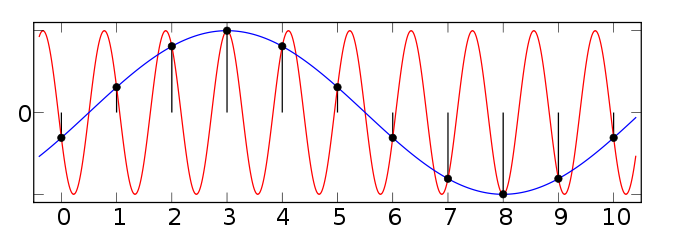
\includegraphics[width=14cm]{third_party_figures/aliasing.png}}

\item Exercise: There is an optical illusion where if you stare at a rapidly spinning object, like a fan or
 car tire, it can appear to be standing still or rotating very slowly.  What do you think is the explanation
 for this?

\item Modes can also alias from positive to negative frequency.
 A sinusoid with $k=N-1$ aliases to $k=-1$, a sinusoid with $k=N-2$ aliases to $k=-2$, and so on.

 So far, we have written the Fourier series as a sum from $k=0$ to $(N-1)$:
\be
  x_j = \sum_{k=0}^N \tx_k e^{(2\pi i/N) jk}  \label{eq:DFT_unaliased}
\ee
 However, because of aliasing, we could equivalently define the Fourier series with the
 sum running over a suitable range of positive and negative $k$, say:
\be
 x_j = \left\{ \begin{array}{cl}
  \sum_{k=-(N-1)/2}^{(N-1)/2} \tx_k e^{(2\pi i/N) jk}  & \mbox{ if $N$ is odd} \\
       \sum_{k=-N/2+1}^{N/2} \tx_k e^{(2\pi i/N) jk}  & \mbox{ if $N$ is even} 
 \end{array} \right.  \label{eq:DFT_aliased}
\ee
 Is it clear why the two forms are equivalent?
 If we consider a term with negative $k$ (say $k=-1$) both the Fourier coefficient $\tx_k$
 and the sinusoid $\exp((2\pi i / N) jk)$ are equal to the same quantities evaluated at positive $k$
 (in this case $k=N-1$).
 It is simply a matter of convention whether we choose to call the mode a ``$k=-1$'' mode
 or a ``$k=N-1$'' mode.  The two are aliases for each other.

 In code, it is convenient to think of the Fourier coefficients $\tx_k$ as being defined for
 $k=0, 1, \cdots, N-1$, and represented by a length-$N$ arrray as in Eq.~(\ref{eq:DFT_unaliased}).

 However, when interpreting the Fourier coefficients $\tx_k$, it makes more sense to think of
 the Fourier modes as being defined over a symmetric range of frequencies as 
 in Eq.~(\ref{eq:DFT_aliased}).\footnote{A convenient accident of python syntax for indexing
   arrays is that ``aliasing happens automatically'', in the following sense.
   Suppose that we call {\tt numpy.fft.fft()} and get the Fourier transform $\tx_k$ represented
   as 1D array {\tt a} of length $N$.  Now suppose that we access the array at a negative index: {\tt a[-1]}.
   In python, negative indices ``count down'' from the end of the array, so {\tt a[N-1]} is returned.
   This is what we wanted, since $k=1$ and $k=N-1$ are aliases.  In other, if we naively index
   arrays with negative indices, then python will automatically supply the proper aliasing.}

 With this aliasing convention, the Fourier transform $\tx_k$ is defined in a band of frequencies 
 $-\nu_* \le \nu \le \nu_*$, where $\nu_* = N / (2 T) = 1 / (2 \Delta t)$.  
 The cutoff frequency $\nu_*$ is called the ``Nyquist frequency''.
 It is the maximum possible frequency for given sampling rate, in the sense that any mode whose
 frequency is larger than $\nu_*$ will be aliased into the band $-\nu_* \le \nu \le \nu_*$.

\item So far we have defined the Fourier transform for a complex-valued time series $x_j$.
 However, in the examples we'll consider, $x_j$ will be real-valued.  In this case, the Fourier
 transform $\tx_k$ will be complex-valued, but it will satisfy the following condition.

 Exercise: If $x_j$ is real-valued, then its Fourier transform satisfies $\tx_{-k} = \tx_k^*$.
 Conversely, given a sequence $\tx_k$ which satisfies this condition, its inverse Fourier transform
 $x_j$ is real-valued.

 This shows that for a real time series, the negative-frequency Fourier coefficients contain the same information
 as the positive-frequency coefficients, so we can just ignore them and think of the Fourier coefficients as
 defined in the band $0 \le \nu \le \nu_*$.

\item [ Say something about periodic vs non-periodic boundary conditions here ]

\item Summarizing the discussion so far, when we take the Fourier transform of a real-valued time series $x_j$,
  we get a complex-valued array of length $N$.  The second half of this array corresponds (under aliasing)
  to negative frequencies, which contain redundant information.  The first half of the array corresponds
  to a band of frequencies ranging from $\nu=0$ (the DC mode) to $\nu = 1/(2\Delta t)$ (the Nyquist frequency).
  The spacing between frequencies is $\Delta \nu = 1/T$.

\item Now let's start looking at some examples!
  If you run the python script {\tt scripts/simulate-1d-examples.py}, some example time series will be written to disk.
  Let's start with {\tt gaussian\_white\_noise.txt}.
  ``Gaussian white noise'' is a time series $x_j$ where every sample is an independent Gaussian random number.

  Read this file and take its Fourier transform $\tx_k$.

  Let's study the behavior of the amplitudes $|\tx_k|$ as a function of $k$,
  disregarding the complex phases for now.
  If you simply plot $|\tx_k|$ as a function of $k$, there will be a lot of statistical scatter
  from one $k$-value to the next, and the plot will be difficult to interpret.
  Therefore, to make a nice plot, you should group the $k$-values into bins (say 32), and average 
  over $k$-values in the bin in order to reduce statistical noise.

  It's conventional to plot the squared amplitude $|\tx_k|^2$ rather than the amplitude $|\tx_k|$.
  As a bit of terminology, the squared amplitude $|\tx_k|^2$ (usually with bin-averaging applied)
  is called the ``power spectrum'' of the time series.
 
  Exercise: Make a plot of the power spectrum of Gaussian white noise, 
  as a function of $k$.\footnote{For plotting from python, I recommend {\tt matplotlib}.}
  How does the power spectrum depend on $k$?

\item You should now have code which can plot the power spectrum, given a text file containing
 a time series.  Let's use it to look at the power spectrum of a few more examples.

 Exercise: The file {\tt gaussian\_random\_walk.txt} contains a ``Gaussian random walk'', i.e.~a time
 series in which each sample $x_j$ is generated from the previous sample $x_{j-1}$ by adding
 a Gaussian random number.  How does its power spectrum compare to the Gaussian white noise case?

 As an aside, the random walk is an example of what might be called ``red noise'': a time series
 with long-timescale drifts relative to the white noise case.  A real-world noisy time series, for
 example the electric field measured at an antenna in a radio telescope, might be roughly modeled
 as the sum of a white noise contribution from thermal fluctuations and a red noise contribution
 from random drifts in amplifier gains.

\item Exercise: {\tt noisy\_sine\_wave.txt} contains a sine wave with a small amount of Gaussian 
  white noise added.  Can you guess what its power spectrum might look like?
  Confirm your guess by making a plot.

\item Exercise: {\tt square\_wave.txt} contains a ``square wave'': a signal which periodically switches
  from -1 to +1.  Can you guess in advance what its power spectrum might look like?  Check by plotting it.

\item [ Von Mises example ]

\item [ Exercise/comment on sine/cosine example ]

\end{itemize}

%\begin{figure}
%\centerline{\includegraphics[width=14cm]{x.pdf}}
%\caption{xxx}
%\label{fig:xxx}
%\end{figure}

% Note: Syntax for clipping a figure is
% \includegraphics[trim={5cm 0 0 0},clip,...]
%  where ordering is <left> <lower> <right> <upper>

% \section*{Acknowledgments}
%
% Research at Perimeter Institute is supported by the Government of Canada
% through Industry Canada and by the Province of Ontario through the Ministry of Research \& Innovation.
% Some computations were performed on the GPC cluster at the SciNet HPC Consortium.
% SciNet is funded by the Canada Foundation for Innovation under the auspices of Compute Canada,
% the Government of Ontario, and the University of Toronto.
% KMS was supported by an NSERC Discovery Grant and an Ontario Early Researcher Award.

% \bibliographystyle{h-physrev}
% \bibliography{xxx}

% \appendix
% \section{Appendix}

\end{document}
